\documentclass[10pt,dvips,twoside,reqno]{amsart} 
\usepackage{epsfig}
\usepackage[authoryear]{natbib} \setlength{\oddsidemargin}{0in}
\setlength{\evensidemargin}{0in} \setlength{\topmargin}{-0.25in}
\setlength{\headheight}{0.1in} \setlength{\headsep}{0.15in}
\setlength{\topskip}{0in} \setlength{\footskip}{0.15in}
\setlength{\textwidth}{6.5in} \setlength{\textheight}{9in}

%differential operators
\newcommand{\grad}{\nabla}
\newcommand{\deld}{\nabla \cdot}
\newcommand{\lap}{\Delta}
%boldface in math mode
\newcommand{\bm}[1]{\mbox{{\boldmath ${#1}$}}}
% vectors and tensors
\renewcommand{\vec}[1]{{\bf #1}}
\newcommand{\gvec}[1]{\mbox{{\boldmath ${#1}$}}}
\newcommand{\ten}[1]{\bar{\bm{#1}}}
%derivatives
\newcommand{\od}[2]{\frac{d {#1}}{d {#2}}}
\newcommand{\ods}[2]{\frac{d^2{#1}}{d {{#2}^2}}}
\newcommand{\pd}[2]{\frac{\partial {#1}}{\partial {#2}}}
\newcommand{\pds}[2]{\frac{\partial^2{#1}}{\partial {{#2}^2}}}
\newcommand{\pdsm}[3]{\frac{\partial^2{#1}}{\partial {#2}\,\partial {#3}}}
%funtional analysis
\newcommand{\abs}[1]{\left| #1 \right|}
\newcommand{\norm}[1]{\left\| #1 \right\|}
\newcommand{\iprod}[2]{\left( #1, #2 \right)}
\newcommand{\dprod}[2]{\left\langle #1, #2 \right\rangle}
%real numbers
\newcommand{\field}[1]{\mathbb{#1}}
\newcommand{\R}{\field{R}}
%funciton spaces
\newcommand{\M}{\mathcal{M}}
%delimiters
\newcommand{\pl}{\left(}
\newcommand{\pr}{\right)}
\newcommand{\sbl}{\left[}
\newcommand{\sbr}{\right]}
\newcommand{\dbl}{\left[\hspace{-0.05cm}\left[}
\newcommand{\dbr}{\right]\hspace{-0.05cm}\right]}
\newcommand{\cbl}{\left\{ }
\newcommand{\cbr}{\right\} }
\newcommand{\eqn}[1]{equation \ref {eq:#1}} 
\newcommand{\Eqn}[1]{Equation \ref {eq:#1}} 
\newcommand{\eqnst}[2]{equations \ref{eq:#1} and \ref{eq:#2}} 
\newcommand{\Eqnst}[2]{Equations \ref{eq:#1} and \ref{eq:#2}} 
\newcommand{\eqns}[2]{equations \ref{eq:#1}--\ref{eq:#2}} 
\newcommand{\Eqns}[2]{Equations \ref{eq:#1}--\ref{eq:#2}}
\newcommand{\msection}[1]{ \vspace{.2in} {\noindent \bf #1}.}
\renewcommand{\for}{\mbox{for}\quad}
%\newcommand{\for}{\mbox{for}\quad}
\newcommand{\argmin}{\mbox{argmin}}
\newcommand{\argmax}{\mbox{argmax}}
\newcommand{\fig}[1]{figure \ref{fig:#1}} 
\newcommand{\Fig}[1]{Figure \ref{fig:#1}} 
\newcommand{\figst}[2]{figures \ref {fig:#1} and \ref {fig:#2}} 
\newcommand{\Figst}[2]{Figures \ref {fig:#1} and \ref {fig:#2}} 
\newcommand{\figs}[2]{figures \ref{fig:#1}--\ref{fig:#2}} 
\newcommand{\Figs}[2]{Figures \ref{fig:#1}--\ref{fig:#2}}
\newcommand{\tab}[1]{table \ref {tab:#1}} 
\newcommand{\Tab}[1]{Table \ref {tab:#1}} 
\newcommand{\tabst}[2]{tables \ref {tab:#1} and \ref {tab:#2}} 
\newcommand{\Tabst}[2]{Tables \ref {tab:#1} and \ref {tab:#2}} 
\newcommand{\tabs}[2]{tables \ref{tab:#1}--\ref{tab:#2}} 
\newcommand{\Tabs}[2]{Tables \ref{tab:#1}--\ref{tab:#2}}
\newtheorem{theorem}{Theorem}
\newenvironment{neqnarray}[1]{\begin{minipage}[t]{6.5in}  \begin{minipage}[b]{1.0in} #1 \end{minipage}  \begin{minipage}[b]{5.5in}\begin{eqnarray}}{\end{eqnarray}\end{minipage}\end{minipage}}
\newcommand{\bneqnarray}[2]{\\ \\ \fbox{\begin{neqnarray}{#1} #2 \end{neqnarray}}\\ \\ \noindent} 

\begin{document}

\begin{center}
  {\bf NOTES ON FLOW AND TRANSPORT IN POROUS MEDIA: DISCRETIZATIONS
    \\}
  Chris Kees\\
  Center for Research in Scientific Computation, Department of Mathematics, North Carolina State University, Raleigh, NC 27695-8205, email: \texttt{chris\_kees@ncsu.edu} \\
  October 4, 2004
\end{center}
\markboth{FLOW AND TRANSPORT IN POROUS MEDIA:
  DISCRETIZATIONS/KEES}{FLOW AND TRANSPORT IN POROUS
  MEDIA:DISCRETIZATIONS/KEES}
\tableofcontents 

\section{Model Equations}

Our goal is solving systems of nonlinear advection-diffusion-reaction
equations of the form
\begin{equation}
  \label{eq:nladrsys}
  \pd{m^i}{t} + \deld \sbl \vec f^i - \sum_{j=1}^{n_c} \ten{a}^{ij} \grad \phi^j \sbr + c^i = s^i \mbox{ in } (0,T] \times U \mbox{ for } i=1,\ldots, n_c
\end{equation}
where $n_c$ is the number of components, $U$ is a bounded open
subset of $\R^3$. The coefficients $m^i$, $\vec f^i$, $\ten{a}^i$, $\phi^i$, and $c^i$
are considered to be functions of $t, \vec x, u^1, \ldots, u^{n_c}$
where $u^i: T \times U \rightarrow \R$ are the components of the
solution. The source term $s^i$ is a function of $t$ and $\vec x$
only. The boundary conditions may be written as
\begin{equation}
  \label{eq:bc}
  G^i(x,t,u^1,\dots,u^{n_c}) = 0 \mbox{ on } (0,T] \times \partial U 
\end{equation}
and usually take the form
\begin{eqnarray}
\sbl \vec f^i - \sum_{j=1}^{n_c} \ten{a}^{ij} \grad \phi^j \sbr \cdot \gvec \nu - f_N &=& 0\mbox{ on } (0,T] \times \partial U_N \\
u^i - u_D &=& 0 \mbox{ on } (0,T] \times \partial U_D
\end{eqnarray}
The initial conditions are
\begin{equation}
  \label{eq:ic}
  u^i(x,0) = u^i_0(x) \mbox{ on } \bar{U}
\end{equation}
We seek to approximate the solution components $u^i$, which lie in
some space of functions $X$ defined on $U_T = (0,T] \times
U$. For a classical solution, if the coefficients are sufficiently
regular, say $C^{\infty}(U_T \times \R^{n_c})$, then we could
define
\begin{equation}
X = C^2_1(U_T) = \cbl u^i: U_T \rightarrow \R | u^i, D_t u^i, D^{\alpha}_x u^i \in C(U_T), |\alpha| =1,2 \cbr  
\end{equation}
We can also think of the equation as an evolution equation on
\begin{equation}
X(t) = \cbl u^i(t) : U \rightarrow \R | u^i, D^{\alpha}_x u^i \in C(U_T), |\alpha| = 1,2, \mbox { and } G(x,t,u^1,\ldots,u^{n_c}) = 0 \cbr  
\end{equation}
so that
\begin{equation}
  \label{eq:classicalEvolution}
  u^i_t = F^i(u^1,\ldots,u^{n_c}) 
\end{equation}
where $F^i: X^{n_c} \rightarrow \R$ and $u^i \in C^1((0,T],X(t))$. The norm on $X(t)$ could be
\begin{equation}
\|u^i(t)\|_{X(t)} = \sup_{x \in U} |u^i(t,x)|
\end{equation}
Instead of seeking classical solutions, various weak formulations of
\eqns{nladrsys}{ic} will be used. 

First consider the steady state equation
\begin{equation}
  \label{eq:steadyState}
  \deld \sbl \vec f^i - \sum_{j=1}^{n_c} \ten{a}^{ij} \grad \phi^j \sbr + c^i = s^i \mbox{ in } U 
\end{equation}
with boundary conditions $G(x,\infty,u^1,\ldots,u^{n_c}) = 0$.
Multiplying \eqn{nladrsys} by a test function $w^i \in
C^{\infty}(U) \rightarrow \R$ and integrating by parts yields
\begin{equation}
  \label{eq:weakSteadyState}
  -\int_{U} \cbl \sbl \vec f^i - \sum_{j=1}^{n_c} \ten{a}^{ij} \grad \phi^j \sbr \cdot \grad w^i + c^iw^i \cbr dU = \int_{U} s^iw^i dU - \int_{\partial U} \sbl \vec f^i - \sum_{j=1}^{n_c} \ten{a}^{ij} \grad \phi^j \sbr w^i \cdot \gvec \nu da \quad \forall w^i
\end{equation}
Usually one takes $w^i$ in $C^{\infty}_c(U)$ (that is the support of $w$ is a compact set contained in $U$). This equation holds on the domain
\begin{equation}
  \label{eq:weakDomain}
  X = \cbl u^i:U \rightarrow \R | \vec f^i, \ten{a}^{ij} \grad \phi^j, c^i, s^i \in L_p(U) \cbr
\end{equation}
where the derivatives are taken in the weak sense. If the coefficients
are smooth then we can take $X$ to be $W^{1,p}(U)$ and the weak
formulation is defined for all $w \in W^{1,p}$.  We can then write
\eqn{weakSteadyState} as
\begin{equation}
  \label{eq:conciseWeakSteadyState}
  -F^i(u^1,\ldots,u^{n_c},w^i) = (s^i,w^i)
\end{equation}
where $F^i:X^{n_c}\times X \rightarrow \R$. The non-steady case can then be
written as
\begin{equation}
  \label{eq:weakEvolution}
  \int_{U} m^i_t w^i dU = F^i(u^1,\ldots,u^{n_c}) + b^i  
\end{equation}
where, for instance, $m^i \in C^1((0,T];X)$,
\begin{equation}
  \label{eq:domainSemiGroup}
  X = \cbl u^i:U \rightarrow \R | \vec f^i, \ten{a}^{ij} \grad \phi^j, c^i, s^i \in L_p(U) \mbox { and } G(t,x,u^1,\ldots,u^{n_c}) = 0\cbr
\end{equation}
and the norm on $X$ is
\begin{equation}
  \label{eq:Lpnorm}
  \| u^i(t) \|_X = \pl \int_U |u^i|^p \pr^{1/p} 
\end{equation}
For linear equations the right hand side of $\eqn{weakEvolution}$ lies
in $(W^{1,p})^*$ so a weaker space for solutions in which
\eqn{weakEvolution} makes sense is to find $u \in L^p(0,T;W^{1,p}(U))$
with $\pd{u}{t} \in L^p(0,T;(W^{1,p})^*)$. In this case it can be
shown that $u \in C([0,T];L^p(U))$ so the boundary conditions can be
specified with $u(0) = u_0$.
 
We can also consider a weakened version in time by considering $w^i \in
C^{\infty}(U_T)$, which yields
\begin{equation}
  \label{eq:weakSpaceTime}
  \int_{U_T} m^i w^i_t + \sbl \vec f^i - \sum_{j=1}^{n_c} \ten{a}^{ij} \grad \phi^j \sbr \grad w^i + c^iw^i dU = \left. \int_{U} m^i_0 dU \right|_0^T+\int_0^T \int_{\partial U} \sbl \vec f^i + \sum_{j=1}^{n_c} \ten{a}^{ij} \grad \phi^j \sbr w^i \cdot \gvec \nu da - \int_{U_T} s^iw^i dU 
\end{equation}
Lastly we consider the case when $U$ is also a function of $t$.  Let
$\vec y = y_1 \vec e_t + y_1 \vec e_{x_1} + y_2 \vec e_{x_2} + y_3
\vec e_{x_3} \in U_T$. Applying the divergence theorem over $U_T =
[0,T] \times U$ we obtain the weak formulation:
\begin{eqnarray}
    \int_{U_T} \sbl \nabla_T \cdot \pl \begin{array}{c} m^i \\ \vec f^i - \sum_{j=1}^{n_c} \ten{a}^{ij} \grad \phi^j \end{array} \pr + c^i \sbr w dy &=& \int_{U_T} sw dy \\
    -\int_{U_T} \pl \begin{array}{c} m^i \\ \vec f^i - \sum_{j=1}^{n_c} \ten{a}^{ij} \grad \phi^j \end{array} \pr \cdot \nabla_T w + c^i w dy &=& -\int_{\partial U_T} \pl \begin{array}{c} m^i \\\vec f^i + \sum_{j=1}^{n_c} \ten{a}^{ij} \grad \phi^j \end{array} \pr w \cdot \gvec \nu_T dS(y) \nonumber \\
&&- \int_{U_T} sw dy
\end{eqnarray}
Now we assume that $U_T$ is described by a smooth invertible
mapping of the form
\begin{equation}
\vec y(\vec z) = \sbl \begin{array}{c} t(\tau) \\
\vec x (\tau, \gvec \xi)
\end{array}\sbr = \sbl \begin{array}{c} T\tau \\
\vec x (\tau, \gvec \xi)
\end{array}\sbr
\end{equation}
so that $\vec y: U^c_T \rightarrow U_T$ with $U^c_T = [0,1] \times U^c$ and $U^c = [0,1]^d$. Changing variables
to $\vec z$ yields
\begin{eqnarray}
-\int_{U^c_T} \pl \begin{array}{c} m^i \\ \vec f^i - \sum_{j=1}^{n_c} \ten{a}^{ij} \grad \phi^j \end{array} \pr \cdot \nabla_T w + c^i w |\ten{J}_y| dz &=& -\int_{\partial U^c_T} \pl \begin{array}{c} m^i \\\vec f^i + \sum_{j=1}^{n_c} \ten{a}^{ij} \grad \phi^j \end{array} \pr w \cdot \gvec \nu_T |\ten{J}_y| dS(z) \nonumber \\
&&-  \int_{U_T} sw |\ten{J}_y| dz
\end{eqnarray}
where 
\begin{equation}
  \label{eq:jacobian}
  \ten{J}_y = \sbl \begin{array}{cccc}
T  & 0 & 0 & 0 \\
\pd{x_1}{\tau} & \pd{x_1}{\xi_1} &  \pd{x_1}{\xi_2} &  \pd{x_1}{\xi_3} \\
\pd{x_2}{\tau} & \pd{x_2}{\xi_1} &  \pd{x_2}{\xi_2} &  \pd{x_2}{\xi_3} \\
\pd{x_3}{\tau} & \pd{x_3}{\xi_1} &  \pd{x_3}{\xi_2} &  \pd{x_3}{\xi_3} 
\end{array} \sbr = \sbl \begin{array}{cc} T & 0 \\
 \pd{\vec x}{\tau} & \ten{J} \end{array} \sbr
\end{equation}
and thus
\begin{equation}
|\ten{J}_y| = T |\ten{J}|
\end{equation}
and 
\begin{equation}
  \label{eq:jacobianInv}
  \ten{J}_y^{-1} = \sbl \begin{array}{cc} \frac{1}{T} & 0 \\
- \frac{1}{T}\ten{J}^{-1}\pd{\vec x}{\tau} & \ten{J}^{-1}
\end{array}\sbr
\end{equation}
To complete the change of variables we need to convert the partial
derivative to $z$ variables and apply a change of basis to the
boundary. It can be shown using the chain rule for partial derivatives
that
\begin{equation}
\grad_y w = \ten{J}^{-t}_y \grad_z y \quad \grad_x \phi = \ten{J}^{-1} \grad_{\xi} \phi
\end{equation}
furthermore $\partial U^c$ is given simply by $\tau = 0,1$, $\xi_1 = 0$, etc. thus
\begin{equation}
\gvec \nu = \pm \ten{J}{-t}_y \vec e_k \for k=1,2,3,4
\end{equation}
Making these substitutions yields
\begin{eqnarray}
-\int_{U^c_T} \sbl \pl  \begin{array}{c} m^i \\ \vec f^i - \sum_{j=1}^{n_c} \ten{a}^{ij}  \ten{J}^{-t} \grad \phi^j \end{array} \pr \right. &\cdot& \left. \ten{J}^{-t}_y \grad_z w + c^i w \sbr |\ten{J}_y| dz = \\
&& -\sum_{k=1} \int_{\partial U^c_T} \pm \pl  \begin{array}{c} m^i \\\vec f^i + \sum_{j=1}^{n_c} \ten{a}^{ij} \grad \ten{J}^{-t}\phi^j \end{array} \pr w \cdot \ten{J}^{-t}_y \vec e_k |\ten{J}_y| dS(z) \nonumber \\
&& -  \int_{U_T} sw |\ten{J}_y| dz
\end{eqnarray}
For the simple structure of $\ten{J}_y$ this yields
\begin{eqnarray}
-T\int_0^1 \int_{U^c}  \sbl m^i \frac{w_\tau}{T} \right. &+&  \left. \pl \ten{J}^{-1} \vec f^i - \frac{1}{T} \ten{J}^{-1}\pd{\vec x}{\tau} - \sum_{j=1}^{n_c} \ten{J}^{-1} \ten{a}^{ij} \ten{J}^{-t} \grad_{\xi} \phi^j  \pr \cdot  \grad_{\xi} w + c^i w \sbr |\ten{J}| d\xi d\tau = \\
&& -\left. \int_{U^c} m^i |\ten{J}| d\xi \right|_0^1 \\
&& -\sum_{k=1}^3 T \left. \int_0^1 \int_{\partial U^c} \pl \ten{J}^{-1} \vec f^i - \frac{1}{T} \ten{J}^{-1}\pd{\vec x}{\tau} - \sum_{j=1}^{n_c} \ten{J}^{-1} \ten{a}^{ij} \ten{J}^{-t} \grad_{\xi} \phi^j  \pr \cdot \vec e_k |\ten{J}| dS(\xi)d\tau \right|_{\xi_k=0}^{\xi_k=1}\nonumber \\
&& -  T \int_0^1 \int_{U^c} sw |\ten{J}| d\xi d\tau
\end{eqnarray}
or simply
\begin{eqnarray}
\int_0^1 \int_{U^c}  \sbl \hat{m}^i w_\tau + \pl \sum_{j=1}^{n_c} \hat{\ten{a}}^{ij} \grad_{\xi} \phi^j  - \hat{\vec f} \pr \cdot  \grad_{\xi} w + c^i w \sbr d\xi d\tau &=& -\left. \int_{U^c} \hat{m}^i d\xi \right|_{\tau=0}^{\tau=1} \nonumber \\
&& + \sum_{k=1}^3 T \left. \int_0^1 \int_{\partial U^c} \pl \sum_{j=1}^{n_c} \hat{\ten{a}}^{ij} \grad_{\xi} \phi^j  - \hat{\vec f} \pr \cdot \vec e_k dS(\xi)d\tau \right|_{\xi_k=0}^{\xi_k=1}\nonumber \\
&& - \int_0^1 \int_{U^c} \hat{s} w d\xi d\tau
\end{eqnarray}
This is identical in form to the basic space time weak formulation above. 
\section{Poisson's Equation}

\section{One Phase}

\subsection{Numerical Solution}

We start with the steady state solution of the slightly compressible flow equations in a homogeneous domain $\Omega$ with wells approximated as point sources distributed in space given by $\tilde{f}(\vec x)$, which we write simply as
\begin{equation}
-\deld -\ten K \grad \phi = -\tilde{f} (\vec x)
\end{equation}
Since $K$ is constant we will write the simple test problem as
\begin{eqnarray}
-\grad^2 u &=& f (\vec x) \quad \mbox{in} \quad \Omega\\
u &=& 0 \quad \mbox{on} \quad \partial \Omega
\end{eqnarray}
which is the Poisson equation. 

\subsubsection{1D solution}

Let $\Omega = (0,1)$ and $X={x_0=0,\ldots,x_{N+1}=1}$ be a partition of
$\Omega$. We define the functions $\psi_{i},i=1,\ldots,N$ by
\begin{equation}
\psi_i = \cbl \begin{array}{cl} 
x = 0 & x < x_{i-1} \\
\frac{x - x_{i-1}}{x_{i} - x_{i-1}} & x_{i-1} \leq x < x_i \\
\frac{x_{i+1} - x}{x_{i+1} - x_{i}} & x_{i} \leq x \leq x_{i+1} \\
x = 0 & x > x_{i+1} 
\end{array} \cbr
\end{equation}
Let $V_h = \mbox{span}\cbl \psi_1,\ldots,\psi_N \cbr = \cbl w |
w \in C^0(0,1),w(0)=w(1)=0,w|_{(x_i,x_{i+1})} \in P_1,i=0,\ldots,N \cbr$.

Later it we will find it more convenient to express the basis functions on each element (interval). Let $L_i=x_i-x_{i-1}$
\begin{eqnarray}
\psi_{i,0} &=& \frac{x - x_{i-1}}{L_i} \\
\psi_{i,1} &=& \frac{x_i - x}{L_i} 
\end{eqnarray}
\begin{eqnarray}
(\psi_{i,0})_x &=& \frac{1}{L_i} \\
(\psi_{i,1})_x &=& \frac{-1}{L_i} 
\end{eqnarray}

The discrete variational problem is to find $U \in V_h$ such that
\begin{equation}
\int_0^1 U_x V_x dx = \int_0^1 f V \quad \mbox{for all} \quad V \in V_h
\end{equation}
Since the $\psi$ are a basis for $V_h$ we can write $U = \sum_{i=1}^N U_i \psi_i$. The discrete variational problem is then equivalent to 
\begin{equation}
\sum_{i=1}^{N} U_{i} \int_0^1  (\psi_{i})_x (\psi_{j})_x dx = \int_0^1 f \psi_j \quad \mbox{for} j=1,\dots,N
\end{equation}
We can also break up the integral into the elements (intervals) so that
\begin{equation}
\sum_{k=0}^{N} \int_{x_k}^{x_{k+1}} (\sum_{i=1}^{N} U_i (\psi_i)_x)(\psi_j)_x dx = \sum_{k=0}^{N} \int_{x_k}^{x_{k+1}} f \psi_j dx \quad \mbox{for} j=1,\dots,N
\end{equation}
Using this form we can write the $k$-th element stiffness matrix (symmetric) as
\begin{eqnarray}
\hat{m}_{0,0} &=& \int_{x_k}^{x_{k+1}} (\psi_{k,0})_x^2 dx = 1/L_i \\
\hat{m}_{0,1} &=& \int_{x_k}^{x_{k+1}} (\psi_{k,0})_x (\psi_{k,1})_x dx = -1/L_i\\
\hat{m}_{1,1} &=& \int_{x_k}^{x_{k+1}} (\psi_{k,1})_x^2 dx = 1/L_i
\end{eqnarray}
We can also calculate the global stiffness matrix and load vector directly as
\begin{eqnarray}
m_{i,i} &=& \int_0^1  (\psi_{i})_x (\psi_{i})_x dx = \frac{1}{x_i - x_{i-1}} +\frac{1}{x_{i+1} - x_{i}} \\
m_{i,i+1} &=& \int_0^1  (\psi_{i})_x (\psi_{i+1})_x dx = \frac{-1}{x_{i+1} - x_{i}} \\
m_{i,i-1} &=& \int_0^1  (\psi_{i})_x (\psi_{i-1})_x dx = \frac{-1}{x_{i} - x_{i-1}} \\
f_i &=& \int_0^1 f \psi_i dx
\end{eqnarray}
and $M = \cbl m_{i,j} \cbr, U = u_i, F = f_i$. We can write the problem as
\begin{equation}
M U = F
\end{equation}
For a regular partitioning where $x_i = ih$ this is simply
\begin{equation}
\frac{1}{h} \cbl \begin{array}{ccccc}
 2 & -1 &  0 &  0 & \cdots \\
-1 &  2 & -1 &  0 & \cdots \\
 0 & -1 &  2 & -1 & 0 
\end{array} \cbr
U 
= F
\end{equation}

Now we repeate using 
\begin{equation}
W_h = \cbl w | w \in C^0(0,1),w(0)=w(1)=0,w|_{(x_{i-1},x_{i})} \in \mathcal{P}_2,\cbr
\end{equation}
We need to find a basis for this space. Each $\mathcal{P}_2$ function is specified uniquely by its value at three points. Thus we can write any function in $W_h$ uniquely  on $[x_{i},x_{i+1}]$ if we know it's values at $x_i,\frac{x_i + x_{i+1}}{2},x_{i+1}$. If we let $x_{i+1/2}=\frac{x_{i+1} + x_i}{2}$ then we can define
\begin{eqnarray}
\phi_{i+1,0} &=& \frac{(x - x_{i})(x_{i+1} - x)}{(x_{i+1/2} - x_{i})(x_{i+1} - x_{i+1/2})} \\
\phi_{i+1,1} &=& \frac{(x - x_{i+1/2})(x_{i+1} - x)}{(x_{i} - x_{i+1/2})(x_{i+1} - x_{i})} \\
\phi_{i+1,2} &=& \frac{(x - x_{i})(x_{i+1/2} - x)}{(x_{i+1} - x_{i})(x_{i+1/2} - x_{i+1})} 
\end{eqnarray}
By substituting for $\frac{x_{i+1} + x_i}{2}=x_{i+1/2}$ and $L_i=x_{i+1} - x_{i}$ we can get these in a more convenient form
\begin{eqnarray}
\phi_{i+1,0} &=& \frac{1}{L^2_i}\sbl(x-x_i) + (x - x_{i+1}) \sbr(x-x_1) \\
\phi_{i+1,1} &=& \frac{-4}{L^2_i}(x-x_i)(x-x_{i+1})\\
\phi_{i+1,2} &=& \frac{1}{L^2_i}\sbl(x-x_i) + (x - x_{i+1}) \sbr(x-x_0)
\end{eqnarray}
We'll also need the first derivatives
\begin{eqnarray}
(\phi_{i+1,0})_x &=& \frac{1}{L^2_i}\sbl(x-x_i) + 3(x - x_{i+1}) \sbr\\
(\phi_{i+1,1})_x &=& \frac{-4}{L^2_i} \sbl(x-x_i) + (x-x_{i+1}) \sbr\\
(\phi_{i+1,2})_x &=& \frac{1}{L^2_i}\sbl3(x - x_{i}) + (x-x_{i+1}) \sbr
\end{eqnarray}
and the second derivatives
\begin{eqnarray}
(\phi_{i+1,0})_x &=& \frac{4}{L^2_i}\\
(\phi_{i+1,1})_x &=& \frac{-8}{L^2_i}\\
(\phi_{i+1,2})_x &=& \frac{4}{L^2_i}
\end{eqnarray}

We can then define a basis for $W_h$ as
\begin{eqnarray}
\phi_1 &=& \phi_{1,1} \\
\phi_j &=& \cbl \begin{array}{ll}
\begin{array}{ll}
\phi_{j/2,2} & x_{j/2-1} \leq x \leq x_{j/2} \\
\phi_{j/2+1,0} & x_{j/2} \leq x \leq x_{j/2+1} \\
\end{array} & j \quad \mbox{even} \\
\phi_{(j+1)/2,1}  & j \quad \mbox{odd}
\end{array}\cbr \\
\phi_{2N+1} &=& \phi_{N+1,1}
\end{eqnarray}
Then $\phi_j, j=1,\ldots,2N+1$ spans $W_h$ by construction. The finite dimensional variational problem is then
\begin{equation}
 \int_0^1  \sum_{j=1}^{2N} U_{j} (\phi_{j})_x (\phi_{k})_x dx = \int_0^1 f \phi_k \quad \mbox{for} k=1,\dots,2N
\end{equation}
which can be broken up over the intervals as
\begin{equation}
 \sum_{i=0}^{N} \int_{x_{i}}^{x_{i+1}}  \sum_{j=1}^{2N} U_{j} (\phi_{j})_x (\phi_{k})_x dx = \sum_{i=0}^{N} \int_{x_{i}}^{x_{i+1}}f \phi_k \quad \mbox{for} k=1,\dots,2N
\end{equation}
On each interval the only nonzero contributions to the interval come from the element basis functions
\begin{eqnarray}
&& \int_0^{x_1} \sbl U_1 (\phi_{1,1})_x + U_2 (\phi_{1,2})_x \sbr \phi_k + \\
&& \sum_{i=2}^{N} \int_{x_{i}}^{x_{i+1}}  
\sbl U_{2i-2} (\phi_{i+1,0})_x+ U_{2i-1} (\phi_{i+1,1})_x + U_{2i} (\phi_{i+1,2})_x \sbr (\phi_{k})_x dx + \\
&& \int_{x_N}^1 \sbl U_{2N} (\phi_{N+1,0})_x + U_{2N+1} (\phi_{N+1,1})_x \sbr \phi_k \\
&&= \sum_{i=0}^{N} \int_{x_{i}}^{x_{i+1}}f \phi_k \quad \mbox{for } k=1,\dots,2N
\end{eqnarray}
Since $\phi_k$ can only have support on $[x_i,x_{i+1}]$ if it is one of the element basis functions $\phi_{i+1,*}$ we need only compute the $3 \times 3$ symmetric element matrix $m^{i+1}$
\begin{eqnarray}
m_{0,0} = \int_{x_i}^{x_{i+1}} (\phi_{i+1,0})_x^2 dx &=& \frac{1}{L^4_i} \sbl a(x) + 6b(x) + 9c(x) \sbr\\
m_{1,1} = \int_{x_i}^{x_{i+1}} (\phi_{i+1,2})_x^2 dx &=& \frac{1}{L^4_i}\sbl a(x) + 2b(x) + c(x) \sbr\\
m_{2,2} =\int_{x_i}^{x_{i+1}} (\phi_{i+1,2})_x^2 dx &=& \frac{1}{L^4_i}\sbl 9a(x) + 6b(x) + c(x) \sbr\\
m_{0,1} = \int_{x_i}^{x_{i+1}} (\phi_{i+1,0})_x (\phi_{i+1,1})_x dx &=& \frac{1}{L^4_i}\sbl a(x) + 4b(x) + 3c(x) \sbr\\
m_{0,2} = \int_{x_i}^{x_{i+1}} (\phi_{i+1,0})_x (\phi_{i+1,2})_x dx &=& \frac{1}{L^4_i}\sbl 3a(x) + 10b(x) + 3c(x) \sbr\\
m_{1,2} = \int_{x_i}^{x_{i+1}} (\phi_{i+1,1})_x (\phi_{i+1,2})_x dx &=& \frac{1}{L^4_i}\sbl 3a(x) + 4b(x) + c(x) \sbr
\end{eqnarray}
where
\begin{eqnarray}
a(x) &=& (x-x_i)^2 \\
b(x) &=& (x-x_i)(x-x_{i+1})\\
c(x) &=& (x-x_{i+1})^2
\end{eqnarray}
Completing the computation yields
\begin{equation}
m^i = \frac{1}{3L_i}\sbl \begin{array}{ccc}
7 & -8 & 1 \\
-8 & 16 & -8 \\
1 & -8 & 7
\end{array} \sbr
\end{equation}

\msection{Implementation}

We see that $u=sin(k \pi x)$ satisfies the boundary conditions for any integer $k$. By applying $-\Delta$ we find that the source $f$ must be $f=k^2 \pi^2 sin(k \pi x)$. To compute the right hand side of the discrete system we calculate for an arbitrary polynomial basis function $\eta$
\begin{equation}
I_{\eta}(a,b) = \int_a^b k^2 \pi^2 sin(k \pi x) \eta_k dx
\end{equation}
Integrating by parts twice yields (for a basis function of at most second order).
\begin{equation}
I_{\eta}(a,b) = \sbl-k \pi cos(k \pi) \eta + sin(k \pi) \eta_x + \frac{cos(k \pi)}{(k \pi)} \eta_{xx} \sbr_a^b
\end{equation}
Thus for quadratic elements we have
\begin{eqnarray}
F_k &=& I_{\phi_{(k+1)/2,1}}(x_{(k-1)/2},x_{(k+1)/2}) \quad \mbox{ k odd } \\
F_k &=& I_{\phi_{k/2,2}}(x_{k/2-1},x_{k/2}) + I_{\phi_{k/2+1}}(x_{k/2},x_{k/2+1})\quad \mbox{ k even } 
\end{eqnarray}
and for linear basis functions we have
\begin{equation}
F_k = I_{\psi_{k,1}}(x_{k-1},x_{k})+I_{\psi_{k+1,0}}(x_{k},x_{k+1}) \quad \mbox{k=1,\ldots,N}
\end{equation}
To assemble the stiffness matrix we add the element matrices into the global stiffness matrix for quadratic elements we have, using python slice notation
\begin{equation}
M(2*(i-1):2*(i-1)+3,2*(i-1):2*(i-1)+3) = M + m^i \quad i=1,\ldots,N
\end{equation}
For linear elements we have
\begin{equation}
M(2*(i-1):2*(i-1)+2,2*(i-1):2*(i-1)+2) = M + m^i \quad i=1,\dots,N
\end{equation}

For the error we need to calculate the $L_2$ norm using the analytical solution
$u$
\begin{equation}
\pl \int_0^1 (u - \sum U_i \eta_i)^2 dx )^{1/2} \pr
\end{equation}
again dividing the integral over the elements
\begin{equation}
\pl \sum_{i=0}^{N-1} \int_{x_i}^{x_{i+1}} (u - \sum U_i \eta_i)^2 dx  \pr^{1/2}
\end{equation}
\begin{equation}
\pl \sum_{i=0}^{N-1} \int_{x_i}^{x_{i+1}} (u - \sum_{j} U_i^j \eta_i^j)^2 dx  \pr^{1/2}
\end{equation}
\begin{equation}
\pl \sum_{i=0}^{N-1} \int_{x_i}^{x_{i+1}} (u^2 - \sum_j U_i^j \eta_i^j u - 2 \sum_{j > k} U_i^j U_i^k \eta_i^j \eta_i^k + \sum_j  (U_i^j)^2 (\eta_i^j)^2) dx  \pr^{1/2}
\end{equation}
\begin{equation}
\int_0^1 u^2 = \int_0^1 sin^2(k \pi x) dx = \frac{1}{2 k \pi}(k \pi x - sin k \pi x cos k \pi x)|_0^1 = 1/2
\end{equation}
\begin{equation}
U_i^j \int_{x_i}^{x_{i+1}}  \eta_i^j u dx = \sbl-\frac{cos(k \pi)}{k \pi} \eta + \frac{sin(k \pi)}{(k \pi)^2} \eta_x + \frac{cos(k \pi)}{(k \pi)^3} \eta_{xx} \sbr_{x_i}^{x_{i+1}}
\end{equation}
\begin{equation}
2 U_i^j U_i^k \int_{x_i}^{x_{i+1}} \eta_i^j \eta_i^k dx = \mbox{quadrature is exact}
\end{equation}
\begin{equation}
(U_i^j)^2 \int_{x_i}^{x_{i+1}} (\eta_i^j)^2 dx = \mbox{quadrature is exact}
\end{equation}
%\section{Two Phase}

\section{Scalar Advection-Diffusion-Reaction Equations}

As a test problem for ELLAM we'll solve
\begin{equation}
\label{la}
[m(u)]_t + [f(u)]_x + [-D(u) u_x]_x = 0
\end{equation}
on $\Omega_x \times \Omega_t$ where $\Omega_x=[x_l,x_r]$ and $\Omega_t=[0,T]$ with $u(0,t)=0$ and $u(1,t)=0$. The initial conditions are a slug given by
\begin{equation}
u(x,0) = \cbl \begin{array}{cl} 
0 & x \leq x_{sl} - m\\
1 - (x_{sl} - x)/m & x_{sl} - m < x < x_{sl} \\
1 & x_{sl} \leq x \leq x_{sr} \\ 
1 + (x_{sr} - x)/m & x_{sr} < x < x_{sr} + m  \\
0 & x \geq x_{sl} + m
\end{array} 
\cbr \end{equation} 
where $x_{sl}$ and $x_{rl}$ are the left and right bounds of the slug
and $m$ provides the slope of the edges of the slug. We test the
simple linear advection-diffusion problem with $m(u)=u$, $f(u)=uV$,
and $D(u)=D$ as well as the non-Lipschitz Freundlich isotherm where
$m(u) = u + c u^r$ for $0<r<1$. We won't assume anything about these
functional forms in what follows on the implementation of the ELLAM
numerical solution of the problems.

Assuming we know the solution at $t_n$, let $w$ be a test function. We
multiply \ref{la} by $w$ and integrate over $\Omega_x \times
[t_n,t_{n+1}]$: 
\begin{equation} 
\int_0^1 \int_{t_n}^{t_{n+1}} ([m(u)]_t +
[f(u)]_x + (-Du_x)_x)w dt dx =0 
\end{equation} 
We use the following substitutions to integrate by parts: 
\begin{eqnarray}
[m(u)w]_t &=& [m(u)]_t w + m(u) w_t \\
\sbl f(u)w \sbr_x &=& [f(u)]_x w + f(u) w_x \\
\sbl -D(u) u_x w \sbr_x &=& [-D(u) u_x]_x w - D(u) u_x w_x 
\end{eqnarray} 
This yields 
\begin{eqnarray} 
\int_0^1 \int_{t_n}^{t_{n+1}} (\sbl m(u)w \sbr_t &-& m(u) w_t
+ \sbl f(u) w \sbr_x - f(u) w_x + \\
\sbl -D(u) u_x w \sbr_x &-& \sbl -D(u) \sbr
u_x w_x )dt dx =0 
\end{eqnarray} 

Now we constrain the space of test functions.  1) we require that \linebreak
$supp(w(x,t^{n+1}))=[x_{i-1},x_{i+1}]$ and 2) that $w(x,t)$ satisfies

\begin{equation} 
\int_0^1 \int_{t_n}^{t_{n+1}} (- m(u) w_t - f(u) w_x) dt dx =0
\end{equation}

Assuming solutions $u$ are smooth enough this means simply that
$w$ is locally the solution to 

\begin{equation} 
m(u) w_t + f(u) w_x = 0 
\end{equation} 

Thus $w$ is constant along characteristics that are solutions of 

\begin{equation}
\od{x}{t} = \frac{f(u)}{m(u)} 
\end{equation} 

with initial values given either at $t^{n+1}$ (backward
characteristics) or $t^{n}$ (forward characteristics). As long as we
can represent $u$ over the time step we can solve these equations
numerically. Given some guess for $U^{n+1}$ I represent $u(x,t)$ by
\begin{equation}
U(x,t) = U^{n+1}(x) \frac{(t - t_n)}{(t_{n+1} - t_{n})} - U^{n}(x) \frac{(t - t_{n+1})}{(t_{n+1} - t_{n})} 
\end{equation}
This is equivalent to specifying the space-time basis functions for
the solution space as piecewise linear in time. At present I've
implemented tracking of the nodes of the time level $n$ and $n+1$
element nodes, the gauss integration points, and the outlfow boundary
nodes forward(backward) by applying forward Euler over a
user-specified number of steps. I also have the an option for using
piecewise linear interpolation from the backward characteristics in
order to get approximate forward tracked points. This is implemented as
follows: If $(x^*_l,x_l)$ and $(x^*_r,x_r)$ are pairs of nodes and
backtracked nodes of a w-element then forward tracking of gauss points
in the element $[x^*_l,x^*_r]$ are given by the mapping
\begin{equation}
\tilde{x}(x) = x_r \frac{(x - x^*_l)}{(x^*_r - x^*_l)} - x_l \frac{(x - x^*_r)}{(x^*_r - x^*_l)} 
\end{equation}
Assuming we can track points, let $x^*(x^{n+1},t)$ be the solution of
the backward characteristics and $\tilde{x}(x^n,t)$ be the solution of
the forward characteristics these solutions are just $x^{n+1}-vt$ and
$x^n+vt$ in the case m(u)=u and f(u)=vu (linear advection), but I'll
try not to use the formulas since generally $u$ will not be constant
along the $w$ characteristics. At the spatial boundaries I'll also
need the inverse of the characteristics, which I'll denote
$t^{*}(x^{n+1},x)$ (backward) and $\tilde{t}(x^n,x)$. With this
notation we can now finish the integration by parts for the equation
for test function w. In what follows we usually only need a
representation of the solution at the ends of the
time step, which I'll denote $U^n(x)$,$U^{n+1}(x)$. At ${n+1}$ we assume we have a finite element basis for
the $U$ and $W$ spaces and that $w^{n+1}=\phi_i$ is the $i$-th basis function
of the space of test functions.
 
First we drop the terms corresponding to the ``adjoint condition'' on
$w$. I'm also going to leave out the argument (u) on the
nonlinearities sometimes:
\begin{equation} 
\int_0^1 \int_{t_n}^{t_{n+1}} [(mw)_t + (fw)_x - (Du_x w)_x + D u_x w_x ]dt dx =0 
\end{equation} 
Now we'll do each term separately.

\begin{equation} 
\int_0^1 \int_{t_n}^{t_{n+1}} (mw)_t dt dx = \int_0^1 [ m(x,t^{n+1})w(x,t^{n+1}) -m(x,t^{n})w(x,t^{n}) ] dx 
\end{equation}
The first term in the integral is simply 
\begin{equation} 
\int_{x_{i-1}}^{x_{i+1}} m(x,t^{n+1})w(x,t^{n+1}) dx  = \int_{x_{i-1}}^{x_{i+1}} m(U^{n+1}(x)) \phi_i(x) dx
\end{equation} 
This is a standard nonlinear mass term for finite elements that we
evaluate with gauss quadrature and denote $M^{n+1}(U^{n+1})$. For future reference, given a set of $k$ quadrature points and weights, $\{x_k\}_i$ and $\{g_k\}_i$, the integral over the $i$-th element is
\begin{equation}
\int_{x_{i}}^{x_{i+1}} m(U^{n+1}(x)) \phi_i(x) dx \approx \sum_k m(U^{n+1}(x_k)) \phi_i(x_k) g_k
\end{equation} 
We save the $k$ masses $\{m_k=m(U^{n+1}(x_k))\}$ as well as the quadrature weights and points for future calculations. The Jacobian of the $M^{n+1}$ term has the same structure of a standard mass matrix
with components given by
\begin{equation}
\ten {M}^{'}_{i,j}(U^{n+1}) =  \int_{x_{i-1}}^{x_{i+1}} m^{'}(U^{n+1}(x)) \psi_{j} \phi_{i} dx
\end{equation}
For the freundlich isotherm there is a little more algebraic structure that we
might be able to exploit since $m(u) = u + c u^r$. In this case we can
write the mass as 
\begin{equation} 
M^{n+1}(U^{n+1}) = \ten {M}^{l} U^{n+1} + M^{nl}(U^{n+1}) 
\end{equation} 
and thus the Jacobian can be written as 
\begin{equation} 
\ten {M}^{'}(U^{n+1}) = \ten {M}^{l} + \ten {M}^{nl}(U^{n+1})
\end{equation} 
The nonlinear part of the Jacobian can have terms that blow up as
concentrations go to zero because $m'(c)$ is unbounded for some values
of the freundlich exponent. In the code I give options for nonlinear
iterations that use either $\ten {M}^{l}$ or an approximation to $\ten
{M}^{'}$ where we force $m'(0) = 0$ regardless of the freundlich
exponent.

The next term is complicated by the fact that we haven't specified the
support of $w$ at the $t^n$ time level. However, using the fact that
$w$ is constant along characteristics we can backtrack to the $t^n$
time level to find the support in the domain $[x_l,x_r]$. I'm worried
about confusing things later so I'm going a little overboard on the
notation for supp$(w(x,t^n))$, which will be the interval
$[x^*_{l,i-1},x^*_{r,i+1}]$ defined by

\begin{eqnarray}
x^*_{l,i-1} &=& min(max(x_l,x^*(x_{i-1},t^n)),x_r) \\
x^*_{r,i+1} &=& max(min(x_r,x^*(x_{i+1},t^n)),x_l) 
\end{eqnarray} 
I think with these definitions $f$ (the flow direction) can be arbitrary (as long as $x_l <
x_r$). The second term in the integral is then
\begin{equation}
-\int_{x^*_{l,i-1}}^{x^*_{r,i+1}}m(x,t^{n})w(x,t^{n}) dx = - \int_{x_{i-1}}^{x_{i+1}} m(U^{n}(x)) w^{n}(x) dx
\end{equation} 
We want to evaluate $w$ at $t^{n+1}$ so we need to use the forward
characteristics, $\tilde{x}$ (i.e. we're using the fact that $w(x,t^n)
= w(\tilde{x}(x,t^{n+1}),t^{n+1})$):
\begin{equation}
-\int_{x^*_{l,i-1}}^{x^*_{r,i+1}}m(U^{n}(x))w(\tilde{x}(x,t^{n+1}),t^{n+1}) dx 
\end{equation} 

To calculate this integral we find a range of spatial elements at time level $n$ that contains
$[x^*_{l,i-1},x^*_{r,i+1}]$, say $i^*_l,\ldots,i^*_r$.  To simplify the presentation assume
$x_{i^*_l} = x^*_{l,i-1}$ and $x_{i^*_r} = x^*_{r,i+1}$, so that level $n$ boundary of the test function element is exactly the union of a sequence of spatial elements. We have on
hand the gauss weights and points, as well as the corresponding masses
used to calculate the integral over each element from the previous
timestep. Hence, we can compute the integral above as
\begin{equation}
M^{n}(U^{n+1}) = \sum_{j=i^*_l}^{i^*_r} \sum_k m^j_k \phi_i(\tilde{x}(x^j_k)) g^j_k
\end{equation} 
This integral is a function of the unknown solution $U^{n+1}$ only in
that it is used in obtaining the map $\tilde{x}(x)$. The approximation
will conserve global mass to machine precision since $\sum_i \phi_i(x)
= 1$. When the backtracked elements don't allign perfectly with the
elements at $t^n$ it is a simple matter to include only those gauss
points that lie inside the interval. We can also add in other
``strategic'' points to the integration as long as we play games with
the masses and weights used above. Because the nonlinearity enters in
through the tracking we won't attempt to calculate the Jacobian
analytically at this time. Note that it can possibly have a different
sparsity structure than $\ten M^{'}$ because of the tracking may pick
up contributions from many elements for large CFL numbers. A different
space-time structure of $U$ could avoid this.

Now we move to the next term in the integral: 
\begin{equation} 
\int_0^1 \int_{t_n}^{t_{n+1}} (fw)_x dt dx 
\end{equation} 
We can exchange the order of integration and, since the region is
square, we have 
\begin{equation} \int_{t_n}^{t_{n+1}} fw |_{x_l}^{x^r} dt 
\end{equation} 
Hence this term is only nonzero when the support of $w$ is nonzero on
the spatial boundaries over $[t^n,t^{n+1}]$.  We'll consider the left
boundary for $f'>0$ (i.e. the inflow boundary, characteristic speeds
are positive).How we calculate this integral at $x_l$ depends on the
type of boundary condition applied at $x_l$. If a flux boundary
condition is specified then the integral is already in a form we can
use. We need only define the overlap of the support of $w(x,t)$ with
the boundary: 
\begin{eqnarray}
  t^{+}_{i-1} &=& max(min(t^{*}(x^{n+1}_{i-1},x_l),t^{n+1}),t^n) \\
  t^{-}_{i+1} &=& min(max(t^{*}(x^{n+1}_{i+1},x_l),t^{n}),t^{n+1})
\end{eqnarray} 
If $t^{+}_{i-1} = t^{-}_{i+1}$ then this term is zero
(the support of w doesn't intersect the boundary). Otherwise we use
$t^+$ and $t^-$ as the integration bounds. If a Dirichlet condition is
specified on the boundary then by using the inverse of the forward
characteristics we can change from $t$ to $x$ in the integration.
\begin{equation} 
\int_{t^{-}_{i+1}}^{t^{+}_{i-1}} f(x_l,\tilde{t}(x_l,x)) w(x_l,\tilde{t}(x_l,x)) \od{\tilde{t}}{x} dx
\end{equation} 
Using $\od{\tilde{t}}{x} = m/f$ this reduces to
\begin{equation} 
\int_{x_{i-1}}^{min(x_{i+1},x*(x_l,t^{n+1}))}  m(x_l,\tilde{t}(x_l,x)) w(x_l,\tilde{t}(x_l,x))dx 
\end{equation} 
or
\begin{equation} 
\int_{x_{i-1}}^{min(x_{i+1},x*(x_l,t^{n+1}))}  m(x_l,\tilde{t}(x_l,x)) w(x,t^{n+1})dx 
\end{equation} 
If we want to consider the right hand boundary for $f'>0$ then we need to include
some information that is not at the $t^{n+1}$ time level, but I'll
come back to this. In the case of either a Dirichlet or Neumann condition the inflow boundary will lead to a term that is independent of the unknown solution that we label $M_{in,a}$.

Now we move to the first diffusion term:
\begin{equation} 
-\int_0^1 \int_{t_n}^{t_{n+1}} (Du_x w)_x dt dx =0 
\end{equation} 
which is much like the advective term so that it is zero unless $t^{+}_{i-1} \neq t^{-}_{i+1}$ and then we can use either
\begin{equation}
-\int_{t^-}^{t^+} Du_x w dt
\end{equation}
in expression for a total flux or standard Neumann boundary condition or we have
\begin{equation}
-\int_{x^{-}}^{x^{+}} \frac{m D u_x(x_l,\tilde{t}(x_l,x)) w(x_l,\tilde{t}(x_l,x))}{f} dx
\end{equation}
in the case of a Dirichlet condition. I haven't implemented this term
in the current code because it's not necessary for the test problems,
but I'll label it $M_{in,d}(U^{n+1})$ so as not to forget about it.

Lastly we have the the standard diffusion term, but over a space-time element:
\begin{equation} 
\int_0^1 \int_{t_n}^{t_{n+1}} D u_x w_x  dt dx =0 
\end{equation}
If the element is on the interior then we approximate the integral as
\begin{equation}
\Delta t \int_{x_{i-1}}^{x_{i+1}} D u_x w_x |^{n+1} dx
\end{equation}
if the support of w intersects the boundary we use
\begin{equation}
\int_{x_{i-1}}^{x_{i+1}} D u_x w_x |^{n+1} (t^{n+1} - t^{*}(x_l,x))dx
\end{equation}
I should look more closely at what this actually means as a time
discretization. I think we might have enough data to be more precise
with the space-time integral. In any case we can integrate this term using gaussian quadrature to obtain a standard diffusion term $D(U^{n+1})$ and the stiffness matrix/Jacobian:
\begin{equation}
\ten D^{'}_{i,j} = \int_{\Omega} D'(U) (\psi_j)_x (\phi_i)_x dx
\end{equation}

To complete the discretization we need to
handle ``outflow'' boundaries. What we've done thus far is sufficient
for the time level $t^{n+1}$, but we leave out a wedge of the space
time domain when characteristics exit the domain over $[t^n,t^{n+1}]$.
The way to treat this part of the boundary is to construct test
functions based on their values at points along the outflow boundary
that are related in size to the elements at $t^{n+1}$. Using the
characteristic speeds for $w$ to this end we place nodes at $t^{n+1+i}
= t^{n+1} - i \Delta x / v(x_r,t^{n+1+i-1}),i=1,\ldots,n_t$ where
$n_t$ is the integer part of $Cu=v \Delta t / \Delta x$. We then
define the test functions at $w(x_r,t)$ as we defined them at
$w(x,t^{n+1})$. I'll have to run through the integration for these new
test functions, but it should be very similar to the manipulations at
an inlet boundary.

To complete the discretization we need to specify the basis for the
trial and test spaces. I'm currently using standard piecewise linears.
The fully discrete form yields the nonlinear system for the solution
at $t^{n+1}$
\begin{equation}
F(U^{n+1}) = M^{n+1}(U^{n+1}) - M^{n}(U^{n+1}) + M_{in,a} - M_{in,d}(U^{n+1}) + D(U^{n+1}) = 0
\end{equation}
For the test problems we use Dirichlet boundary conditions and ignore the term $M_{in,d}(U^{n+1})$ so we can add in the boundary condition terms explicitly to yield a system for the interior
\begin{equation}
F(U^{n+1}) = M^{n+1}(U^{n+1}) - M^{n}(U^{n+1}) + M_{in,a} + D(U^{n+1}) = 0
\end{equation}
The Newton iterate for this equation is given by
\begin{equation}
U^{n+1}_+ = U^{n+1}_c - (\ten F^{'})^{-1} F(U^{n+1}_c)
\end{equation}
I currently use a stanard LU decomposition to compute the product of
the inverse Jacobian.  Given the difficulty of calculating the
Jacobian of $M^{n}(U^{n+1})$ as well as the term $M^{n+1}(U^{n+1})$ in
the non-Lipschitz case the implementation provides several choices for
approximating $\ten F^{'}$:
\begin{eqnarray}
\ten F^{'}_1 &=& \bar{\ten M}^{n+1} + \ten D \\
\ten F^{'}_2 &=& \ten M^{l,n+1} + \ten D \\
\ten F^{'}_3 &=& \ten D 
\end{eqnarray}
where $\bar{\ten M}^{n+1}$ and $\ten M^{l,n+1}$ are discussed above. 

The initial guess is for now $U_0 = U^{n}$ and the nonlinear iteration
is terminated on small relative residuals so that upon convergence:
\begin{equation}
\| F(U^{n+1}) \| \leq \| F(U_0) \| * \epsilon_r + \epsilon_a 
\end{equation}

The following numerical results were generated for $D=1.0e-3$, $V=1$,
$CFL=2.25$, $c=0.5$, and $r=0.7$ (as in Freundlich $c u^r)$. The
number of elements was $40,80,160$ and therefore $Pe=25,12.5,6.25$.
There is still noticable over/undershoot at Pe=12.5. The number
of nonlinear iterations required on all grids was 3-6 with the
required number decreaing slighly as the number of elements increased.
The nonlinear solver tolerance was 1.0e-6 and global mass balance
error was less than 1.0e-7.
\begin{figure}
\caption{Pe=25}
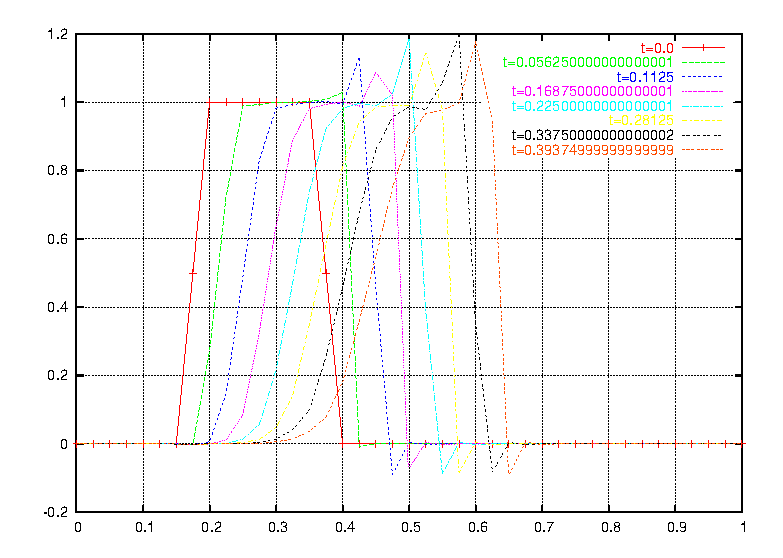
\epsfig{file=fr40.eps}
\end{figure}
\begin{figure}
\caption{Pe=12.5}
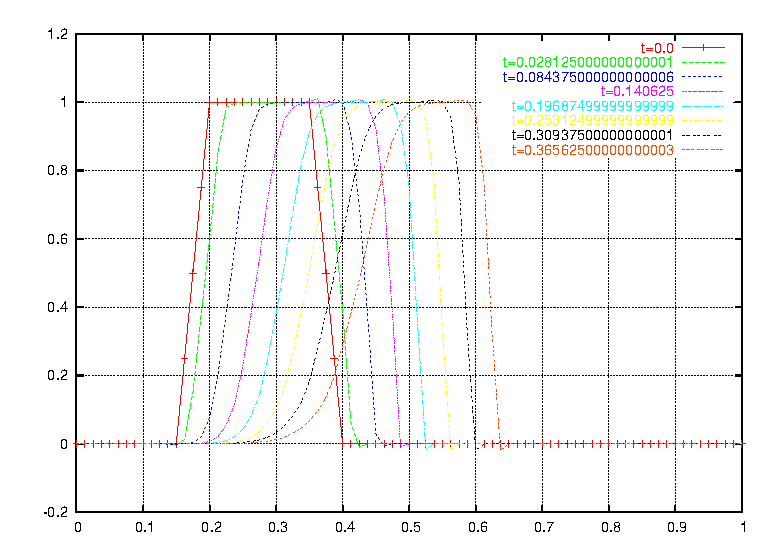
\epsfig{file=fr80.eps}
\end{figure}
\begin{figure}
\caption{Pe=6}
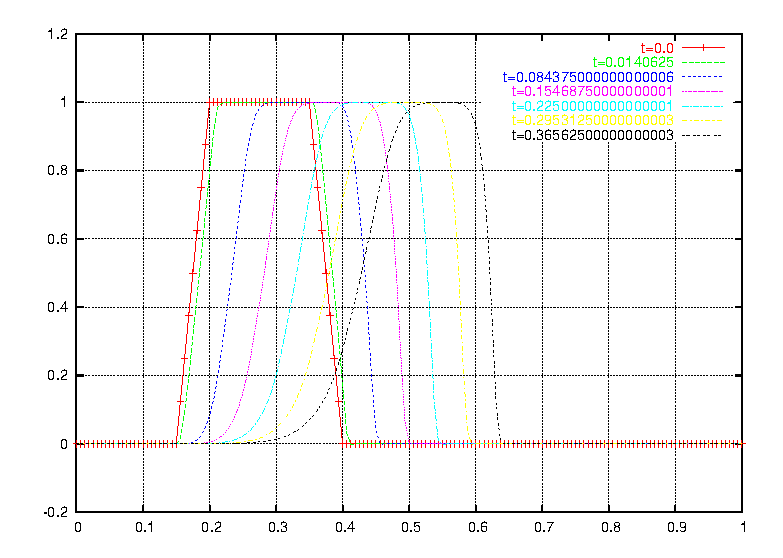
\epsfig{file=fr160.eps}
\end{figure}

\section{Scalar Advection-Diffusion-Reaction Equations-DG}

As a test problem for ELLAM we'll solve
\begin{equation}
[m(u)]_t + [f(u)]_x + [-D(u) u_x]_x = 0
\end{equation}
Following Cockburn we rewrite this as a first order system
\begin{eqnarray}
[m(u)]_t + [f(u)]_x + [-  \sqrt{D(u)} q]_x &=& 0 \\
q  - [g(u)]_x &=& 0 \\
g(u) &=& \int_0^u \sqrt{D(u)} \\
\end{eqnarray}
If we let $\vec u =[u,q]'$, $\vec M(\vec u) =[m(u),0]'$ and $\vec h(\vec u) = [f(u) - \sqrt{D(u)} q,-g(u)]'$ we have simply
\begin{equation}
[\vec M(u)]_t + [\vec h(u)]_x =0
\end{equation}
To get the weak formulation we multiply by a smooth (on I) test function $\vec v=[v_u,v_q]'$ (componentwise multiplication $*$ )and integrate over some spatial domain $I=[x_{j+1/2},x_{j-1/2}]$
\begin{equation}
\int_I [\vec M(u)]_t * \vec v dx + \int_I [\vec h(u)]_x * \vec v dx=0
\end{equation}
and integrate by parts
\begin{equation}
\int_I [\vec M(u)]_t * \vec v dx - \int_I [\vec h(u)] * \vec v_x dx
+\vec h( \vec u(x^-_{j+1/2})) * \vec v(x^-_{j+1/2}) -\vec h( \vec u(x^+_{j-1/2})) * \vec v(x^+_{j-1/2}) = 0 
\end{equation}
where $^+$ and $^-$ are the right and left limits.
To discretize we assume we have a partition of the domain $[0,1]$
given by ${x_{j+1/2}}_j=0^N$ and we use the weak formulation over the
domains $I_j=(x_{j-1/2},x_{j+1/2})$ with the components of the test
and basis functions $\vec u_h, \vec v_h$ taken from the space
\begin{equation}
V_h = \{ v \in L^1(0,1): v|_{I_j} \in P^k(I_j),j=1,\ldots,N \}
\end{equation}
Since the basis and test functions are discontinuous, the semidiscrete
formulations using these functions will not conserve mass globally
unless we require that $\vec h( \vec u(x^+_{j-1/2})) = \vec h( \vec
u(x^-_{j-1/2}))$ (i.e. that the fluxes are continuous). To fulfill this
requirement we define the numerical flux as some function $\hat{\vec
  h}[\vec u(x^+_{j-1/2}),\vec u(x^-_{j-1/2})]$ to be specified later.
With these definitions we obtain the finite dimensional semi-discrete weak formulation: Find $\vec u_h$ such that
\begin{eqnarray}
&\int_{I_j} [\vec M(\vec u_h)]_t * \vec v_h dx - \int_{I_j} [\vec h(\vec u_h)] * \vec v_{hx} dx
+&\\
&\hat{\vec h}[\vec u(x^+_{j+1/2}),\vec u(x^-_{j+1/2})]* \vec v_h(x^-_{j+1/2}) &\\
&-\hat{\vec h}[\vec u(x^+_{j-1/2}),\vec u(x^-_{j-1/2})]* \vec v_h(x^+_{j-1/2}) = 0 &
\end{eqnarray}
for $j=0,\ldots,N$, $\forall v_h \in V_h$. The basis for $V_h$ that we
will use will be $\{1,\frac{x-x_j}{\Delta x_j} \}$ where $x_j =
\frac{x_{j-1/2}+x_{j+1/2}}{2}$ and $\Delta x_j=x_{j+1/2}-x_{j-1/2}$.
The degrees of freedom for each component are then $\{v, \vec v_x\}$
To complete the discretization we need to define the numerical flux. First we define the standard notation for averages and jumps:
\begin{eqnarray}
[p]&=&p^+ -  p^- \\
\bar{p} &=& \frac{1}{2} (p^+ + p^-) \\
\end{eqnarray}
We define the integral transform of the flux function as we did with the square of the diffusion coefficient above:
\begin{equation}
\phi = \int_0^u f(s) ds 
\end{equation}
Now we define the numerical flux as
\begin{equation}
\hat{\vec h} = 
\left\{
\begin{array}{c}
\frac{ \left[ \phi \right] }{ \left[ u \right] } - \frac{ \left[ g(u) \right] }{ \left[ u \right] } \bar{q} \\
- \bar{g(u)} 
\end{array}
\right\}
- \vec C 
\left\{
\begin{array}{c}
\left[ u \right] \\
\left[ q \right] 
\end{array}
\right\}
\end{equation}
The actual entries of C will determine numerical flux. We let
\begin{equation}
\vec C = \left\{
\begin{array}{cc}
\frac{|f'(u)|}{2} & -\frac{\sqrt{D(u)}}{2} \\
\frac{\sqrt{D(u)}}{2} & 0 
\end{array}
\right\}
\end{equation}
For the case $f(u) = c$, $D(u)=a$ (linear advection/diffusion)
\begin{equation}
\hat{\vec h} = 
\left\{
\begin{array}{c}
\frac{c}{2} (u^+ + u^-)  - \frac{\sqrt{a}}{2} (q^+ + q^-)\\
- \frac{\sqrt{a}}{2}(u^+ + u^-) 
\end{array}
\right\}
-  \left\{
\begin{array}{c}
\frac{|c|}{2}(u^+ - u^-) - \frac{\sqrt{a}}{2}(q^+ - q^-) \\
\frac{\sqrt{a}}{2}(u^+ - u^-)
\end{array}
\right\}
\end{equation}
This is upwinding for the advection and supposedly the standard 3
point stencil for diffusion if we use $P^0$ elements.

\bibliographystyle{alpha} \bibliography{mp}
\end{document}









